\documentclass[]{article}
\usepackage{indentfirst}
\usepackage{listings}
\usepackage{xcolor}
\usepackage[cp1250]{inputenc}
\usepackage{graphicx} 
\usepackage{hyperref}

\colorlet{punct}{red!60!black}
\definecolor{delim}{RGB}{20,105,176}
\colorlet{numb}{magenta!60!black}


\lstdefinelanguage{json}{
	basicstyle=\normalfont\ttfamily,
	numbers=left,
	numberstyle=\scriptsize,
	stepnumber=1,
	numbersep=8pt,
	showstringspaces=false,
	breaklines=true,
	frame=lines,
	literate=
	*{0}{{{\color{numb}0}}}{1}
	{1}{{{\color{numb}1}}}{1}
	{2}{{{\color{numb}2}}}{1}
	{3}{{{\color{numb}3}}}{1}
	{4}{{{\color{numb}4}}}{1}
	{5}{{{\color{numb}5}}}{1}
	{6}{{{\color{numb}6}}}{1}
	{7}{{{\color{numb}7}}}{1}
	{8}{{{\color{numb}8}}}{1}
	{9}{{{\color{numb}9}}}{1}
	{:}{{{\color{punct}{:}}}}{1}
	{,}{{{\color{punct}{,}}}}{1}
	{\{}{{{\color{delim}{\{}}}}{1}
	{\}}{{{\color{delim}{\}}}}}{1}
	{[}{{{\color{delim}{[}}}}{1}
	{]}{{{\color{delim}{]}}}}{1},
}

%opening
\title{Why Avro API is the best choice?}
\author{Adrian Strugala}

\begin{document}

\maketitle

\section{Intruduction}

Hi! I am a software developer working in C\# .NET environment. I'm focused mostly on the backend side of the applications. That means I am delivering the data. Fetching the data. Synchronizing the data. Downloading the data. Checking data quality. Pulling the data. Mixing together data from various sources to produce new data. I think you know what I am talking about.

Fortunately, I am living in a microservice world. The data is well organized. The flag project of my company is build of 40-50 services. Each of them exposes from 5 up to 100 API endpoints. Even my side project is build of 6 services, 20 endpoints in total. I am using 3rd party APIs, public APIs, and open APIs. I mean - I know how to communicate between microservices. I do this every day.

Believe me or not, services love to talk to each other. They do this without any break. All the time. That's good. My customers are able to see the data, manipulate it and delete it. Background jobs are generating reports, documents and whatever they want. The problem starts, when the communication slows down the services and they are not able to play their role correctly.


\section{The problem}

Some time ago developers in my company were kindly asked to try to not call on-premise microservices more than it's needed. Surprisingly problem was the local internet bandwidth throughput. Funny or not, the solution from management was really to reduce traffic between microservices.

A few days later I heard a conversation between my colleague and his product owner. The PO asked If there is any quick-win on how to improve response time of his service. It wasn't that bad - just a little bit to slow for the users. The colleague started to explain what's the root cause of the problem: his service was fetching data from one API, then another, then 3rd one, authorizing and validating in the meantime. That means service A response time was strongly dependent on services B, C, D, and E. Then colleague as a great professionalist started to enumerate possible solutions: cache part of the data, go in the direction of CQRS and Event Sourcing - start pre- generating view models as soon as the data changes. His answers were right. But caching in live-APIs is sometimes impossible. Implementation of Event Sourcing is very, very expensive in the existing environment.


I thought about those problems and I found out one, really simple solution which bringed 3 main benefits:
\begin{itemize}
	\item Decrease the microservices communication time
	\item Reduce the network traffic 
	\item Increase security between microservices
\end{itemize}


First things first, though. I'll start with a few words about why we are all in love with Json.


\section{Why Json is amazing}
That's simple - just try to imagine communication without Json. What would you miss the most? The clear and easily readable format? Consistent data model? Maybe the number of tools you can use to parse, read or edit Jsons and even generate it automatically from C\# models?

If fact Json has only one disadvantage that comes to my mind - every response and request is sent as plain text. Sometimes it's not a big deal, but in other cases response time of not compressesd nor encoded Json API could be a real problem.  

\section{Why Avro is better}

Avro file is build of few pieces:
\begin{enumerate}
	\item Magic number
	\item Chosen codec (null in example)
	\item Schema of the data written in Json format
	\item The data itself compressed to binary representation
\end{enumerate}

An example of exactly the same data:

Json:

\begin{lstlisting}[language=json,firstnumber=1]
[
	{
		"minPosition": 188,
		"hasMoreItems": true,
		"itemsHtml": "items_html6e64c2b9-dc87-4be3-b8ba-eca0da96ce78",
		"newLatentCount": 85,
		"itemIds": [
		174,
		43,
		249
		],
		"isAvailable": false
	},
	{
		"minPosition": 160,
		"hasMoreItems": true,
		"itemsHtml": "items_htmlaa233d3b-d6ea-41ff-b50f-f099c0c79991",
		"newLatentCount": 163,
		"itemIds": [
		60,
		153,
		131
		],
		"isAvailable": false
	}
]
\end{lstlisting}

Avro:
\begin{lstlisting}[language=json,firstnumber=1]
Objavro.codecnullavro.schema¨{"type":"array","items":{"type":"record","name":"Dataset","fields":[{"name":"minPosition","type":"int"},{"name":"hasMoreItems","type":"boolean"},{"name":"itemsHtml","type":["null","string"]},{"name":"newLatentCount","type":"int"},{"name":"itemIds","type":{"type":"array","items":"int"}},{"name":"isAvailable","type":"boolean"}]}} /Âźľ)|ř OČëHE řř\items_html6e64c2b9-dc87-4be3-b8ba-eca0da96ce78ŞÜVň  Ŕ\items_htmlaa233d3b-d6ea-41ff-b50f-f099c0c79991Ćx˛†   /Âźľ)|ř OČëHE
\end{lstlisting}

It doesn't look really different here. But imagine very, very long Json. The size of the file would increase lineary with amount of records. While for Avro header and schema stays the same - what increases is amount of encoded and well compressed data.

Avro format inherits redability of Json. Note the schema representation - it could be easily read and extracted from the content. In real life cases this is very helpful. During integration tests I can call an API, and read just schema for the data model - to prepair my classes for deserialization.

Take a look at the data - you are not able to read it at first glace. And that's also a benefit. API responses could be easly catched by network tools. You can even peek the responses in internet browsers. And from time to time happens, that someone spots the data that shouldn't be read by unauthorized person. Keeping data encoded increases security of the solution. Reading Avro is not a big problem for motivated person, but reduces probability of accidential data leaks.

In a real world case API responses are usually a little bit more complex than in this example. How beneficial is serialization using Avro in comparison to Json? 2 times for this example. 3 times for simple API responses. I was able to reach 50 times using right codec for nested model structures containing huge amount of data.

\section{My benchmark results}

Enought talking, lets now focus on numbers. Screen below shows data compressed with different formats and encoding. Take carefull look at the sizes. Json file, which size is about 10 000 KB was compressed to Avro file occupying about 2 500 KB (that's 4 times smaller). 

One of the greates features of Avro format is possiblity to choose codec type (compression algorithm in fact) used for serialization of the data. In this examples GZip and Deflate encodings are clear winners. Enabling one of them decreases file size to only 200 KB - this means: 50 time less than Json.

\begin{figure}[h]
	\centering
	
\includegraphics[width=\textwidth]{size_comparison}
	\caption{Comparison of the same file compressed with different options}
\end{figure}

At this point let me introduce library that I've created in purpose of handling serializaiton and deserialization C\# objects to Avro format: AvroConvert: 
\href{https://github.com/AdrianStrugala/AvroConvert}{Github page}.
I've strongly focused on dev workflow and usability of the package. It's interface should be clear and familiar for every user.  

Bechmark below mimics sending API response. Calculates time of serialization of the messege, time for used for transport (based on size) and time of deserialization: 

\begin{figure}[h]
	\centering
	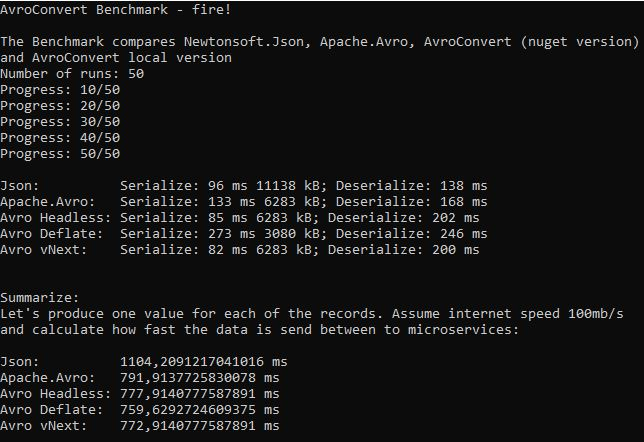
\includegraphics[width=\textwidth]{benchmark}
	\caption{Comparison of result from AvroConvert benchmark}
\end{figure}

Winner in this category is official implemetation of Avro format in the C\# world: Apache.Avro. Unfortunetaly it doesn't support many of key types like: decimal, dictionary, list or Guid.


\section{How to build Avro API}

\section{Useful links}


\end{document}
